Our approach to the problem is the following: \\ 
We create a source node, and to this node we connect $n$ nodes each representing one of the $n$ persons sharing the kitchen (let's call those nodes $P_i$ , $i$ ranging from 1 to $n$). The connecting edges between the source and the $P_i$ nodes initially all have a capacity of $D_i$. Then we create a sink node and to this node we connect $j$ nodes that represent all the days the kitchen is used (let's call those nodes $M_k$, $k$ ranging from 1 to $j$). All edges connecting the days with the sink have a capacity of 1. Then we connect each $P_i$ node with all the $M_k$ nodes that correspond to the days this person has been using the kitchen, again with edges of unitary capacity. When this process is complete, we have our network (Figure \ref{fig:prob2}).\\
\begin{figure}[ht]
\centering
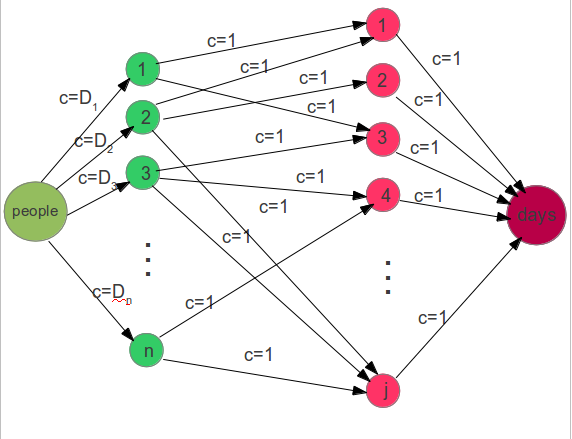
\includegraphics[width=0.75\textwidth]{prob2}
\caption{Our network flow}
\label{fig:prob2}
\end{figure}
\\ 

We apply the Ford-Fulkerson algorithm to the network that we created with the above mentioned procedure, to find the maximum flow of the network. If we can get a maximum flow that equals $j$ that implies there is a valid assignment, such that every day there is exactly one person that will clean the kitchen, without exceeding his capacity $D_i$. The cost of the algorithm is the cost of the maximum flow algorithm. Using the ford-fulkerson algorithm for the maximum flow, we get a complexity of $O(V * \max (flow)) = O(V * j)$ which is polynomial.